\documentclass[11pt,letterpaper]{article}
\usepackage[top=0.85in,left=1.00in,footskip=0.75in]{geometry}
\usepackage[titletoc,page]{appendix}
% Use adjustwidth environment to exceed column width (see example table in text)
\usepackage{changepage}
\usepackage[english]{babel}
\usepackage{booktabs}
\usepackage{siunitx}%Questo serve a caricare il pacchetto delle unità di misura del sistema internazionale%
\usepackage[utf8]{inputenc}
\usepackage{graphicx} 
\usepackage{url}
\usepackage{amsmath}
\usepackage{amssymb}
\usepackage{listings}


\usepackage{keyval}
\usepackage{xcolor}
\usepackage{caption}
\usepackage{tikz}
\usepackage{circuitikz}
\usepackage{authblk}
%\usepackage{hyperref}


\usepackage[lofdepth,lotdepth]{subfig}
% Remove comment for double spacing
%\usepackage{setspace} 
%\doublespacing
% Text layout
%\raggedright
\setlength{\parindent}{0.5cm}
\textwidth 5.25in 
\textheight 8.75in

\usepackage[aboveskip=1pt,labelfont=bf,labelsep=period,justification=raggedright,singlelinecheck=off]{caption}

% Use the PLoS provided BiBTeX style
\bibliographystyle{plos2009}

% Remove brackets from numbering in List of References
\makeatletter
\renewcommand{\@biblabel}[1]{\quad#1.}
\makeatother


\begin{document}
\vspace*{0.30in}

\begin{flushleft}
{\Large
\textbf\newline{\textbf{Decoherence of nonclassical state of a harmonic oscillator}}
}
\newline
% Insert Author names, affiliations and corresponding author email.
\\
Lorenzo Maria Perrone\textsuperscript{1, *}
%Name2 Surname\textsuperscript{2,\textpilcrow},
%Name3 Surname\textsuperscript{2,\textcurrency a},
%Name4 Surname\textsuperscript{2,\ddag},
%Name5 Surname\textsuperscript{2,\ddag},
%Name6 Surname\textsuperscript{2,\Yinyang},
%Name7 Surname\textsuperscript{3,*,\Yinyang}
\\
\bf{1} Department of Physics, EPFL
\\
%\bf{2} Affiliation Dept/Program/Center, Institution Name, City, State, Country
%\\
%\bf{3} Affiliation Dept/Program/Center, Institution Name, City, State, Country
%\\

% Insert additional author notes using the symbols described below. Insert symbol callouts after author names as necessary.
% 
% Remove or comment out the author notes below if they aren't used.
%
% Primary Equal Contribution Note
%\Yinyang These authors contributed equally to this work.

% Additional Equal Contribution Note
%\ddag These authors also contributed equally to this work.

% Current address notes
%\textcurrency a Insert current address of first author with an address update
% \textcurrency b Insert current address of second author with an address update
% \textcurrency c Insert current address of third author with an address update

% Deceased author note
%\dag Deceased

% Group/Consortium Author Note
%\textpilcrow Insert Collaborative Author line here

* E-mail: lorenzo.perrone@epfl.ch
\end{flushleft}

\section{QuTip package for Python}
QuTIp is a very powerful tool to simulate the evolution of quantum mechanical system. In particular, the convention used in its function of time evolution (\textsc{odesolve}, \textsc{mesolve} etc) requires a hamiltonian of the system (for example our harmonic oscillator) plus the definition of jump/collapse operators in the Lindblad form. This is particularly easy to achieve, since such operators can be easily defined (check in the code).\\
Our formulation of the code is somewhat more general: the temperature of the bath can be changed as a parameter (consequently $\gamma_2$ can become relevant) and the ladder/number operators can be extended in a tensor product of many Hilbert spaces: this could be used to simulate the coupling of two or more harmonic oscillator between themselves and with the bath. 
\begin{lstlisting}

#import all the necessary packages
import matplotlib.pyplot as plt
from numpy import *
import qutip.settings 
from qutip import *
from matplotlib import rcParams
rcParams['font.family'] = 'STIXGeneral'
rcParams['mathtext.fontset'] = 'stix'
rcParams['font.size'] = '14'


#setting up of the parameters

N = 4               # number of cavity states from 0 to 3
omega0 = 2* pi     # frequency of the harmonic oscillator
gamma1 = 0.2              # energy relaxation rate of oscillator
gamma2 = 0.05               # dephasing rate of oscillator
n_th = 0.0                # bath temperature

## define ladder operators and number operator for one oscillator system
a  = tensor(destroy(N), qeye(1))
number  = tensor(num(N), qeye(1))

## define Hamiltonian and initial state ##
H0 = omega0 * a.dag() * a  #h bar = 1
 
# tensor product of bath state (ground state) 
and initial state of the oscillator NOT NEEDED IN THE COMPUTATION
psi0 = tensor(fock(N,0), (fock(N,0) + fock(N,3))/sqrt(2))
# reduced density matrix for the oscillator at instant t=0
rho_0 = 0.5*fock_dm(N, 0) + 0.5*fock_dm(N, 3)  

#sm = tensor(qeye(N), destroy(2))
#sz = tensor(qeye(N), sigmaz())
#H  = omega0 * a.dag() * a + 0.5 * epsilon * sz
#+ g * (a.dag() * sm + a * sm.dag())

## define Lindblad jump (collapse) operators
c_ops = []
c_ops.append(sqrt(gamma1*(1+n_th)) * a)     #L1-
c_ops.append(sqrt(gamma1*n_th) * a.dag())   #L1+
c_ops.append(sqrt(gamma2) * number)         #L2

## Evolution of the system ##
tlist = linspace(0, 20, 50)
#rho_t = odesolve(H, psi0, tlist, c_ops) not sure
rho_t = odesolve(H0, rho_0, tlist, c_ops, [])


#Plot results

#this is useful if one wants to plot the wigner functions
#fig, axes = plt.subplots(2,1, figsize=(12,3))
#plot_wigner_fock_distribution(rho_0, fig= fig, ax=axes[0], cmap=cm.RdBu, title="initial state");
#plot_wigner_fock_distribution(rho_t(100), fig= fig, ax=axes[1], title="final state");
#fig.tight_layout()
#plt.show()

rho11 = [];
rho00 = [];
rho22 = [];
rho33 = [];
for i in range(50):
    rho00.append(rho_t[i].data[0,0]);
    rho11.append(rho_t[i].data[1,1]);
    rho22.append(rho_t[i].data[2,2]);
    rho33.append(rho_t[i].data[3,3]);
fig = plt.plot()
plt.plot(tlist, rho00, 's')
plt.plot(tlist, rho11, 's')
plt.plot(tlist, rho22, 's')
plt.plot(tlist, rho33, 's')
plt.title("Amplitudes of diag. elements density matrix")
plt.xlabel("time [seconds]")
plt.ylabel("amplitude")
plt.grid('on')
plt.show()


\end{lstlisting}

\begin{figure}
\centering
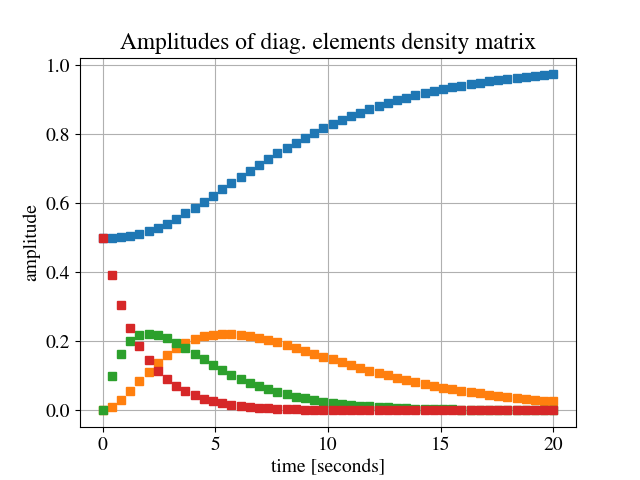
\includegraphics[width=1.0\linewidth]{./lind_lore}
\caption{Simulation of the evolution of the diagonal terms of the density matrix. The parameter $\gamma_1$ and the elapsing time must of course be tuned with each other.}
\label{fig:lind_lore}
\end{figure}

The code can be accessed at \textsc{https://github.com/LorenzoLMP/StatPhys4}.


\end{document}